% An implementable description of the process you chose.
% Make sure the textual description in combination with the BPMN
% model describes your process completely, such that someone else is
% able to implement the control flow perspective, the resource perspective
% and the data perspective. Please make sure the BPMN model is
% readable when the report is printed on A4.
% Workflow patterns Highlight and motivate each workflow pattern
% from Section 2.2 once.
% Soundness Argue that the control flow of the process is sound.
% Please note that the syntactic sugaring and hacks (e.g. the milestone)
% introduced for Bizagi are not considered for the soundness check by
% ProM. An argument that a model is sound could be the combination
% of a check by ProM and a manual analysis of these special parts.

\subsection{Description}
In this section we describe in detail how we model the description of the exercise, as given in \autoref{app:appendix_exercise}.
To make this description easier to understand we will use figures of parts of the model to show how we modeled the process, but it should be possible to understand this without the figures.
A complete overview of the process modeled in Bizagi can be found in \autoref{app:appendix_model1}.

At the start of the process a student requests an application to study in Eindhoven.
This is the start event in our process.
From this start event we move on to the first task which is called \emph{Register request}.
In this task a administrative employee handles the request from the student (by entering it in the system of the TU/e) and the process moves on to two tasks which happen simultaneously.

The first task is done by a mail department employee, which is gathering all the forms which have to be send, disregarding if the request was on time or not, to the new student.
This task is named \emph{Gather standard forms}.
The second simultaneous task was that a mail department employee checks if the request was made on time, if not he adds a request for a motivation letter to the package which will be send to the student.
If the request was on time he does nothing but communicates that the request was on time.
The name of this task is \emph{Add motivation letter request}.

When both these tasks are finished the process goes to the next task, which is \emph{Send enrollment package}.
In this task a mail department employee sends the package to the student.
The next task is \emph{fill out and send back forms}.
In this task the student has to fill out the forms he got and send them back to the university.
If this is done within two weeks the process moves on to the next task.
If this is not done in two weeks, the whole process ends and the request expires.
This is modeled by a timer on the task \emph{fill out and send back forms}, if this timer expires the process continues to an end event.

If the forms were send back on time the next task is \emph{Check if forms are complete}.
In this task an administrative employee checks if all the forms are filled in.
If this is not the case the process goes to the task \emph{Add explanation missing items}.
In this task the mail department employee adds the explanation for the missing items to the package which will be send again.
The process now continues to the point right after that the request was registered in the system.
This also means that a mail department employee checks if the request is still on time or that in this new case a motivation is required.
This is because it is possible that a students first request was just in time for the deadline, but because it is two weeks later now and he has to do it over again the deadline has passed.

\begin{figure}[H]
	\centering
	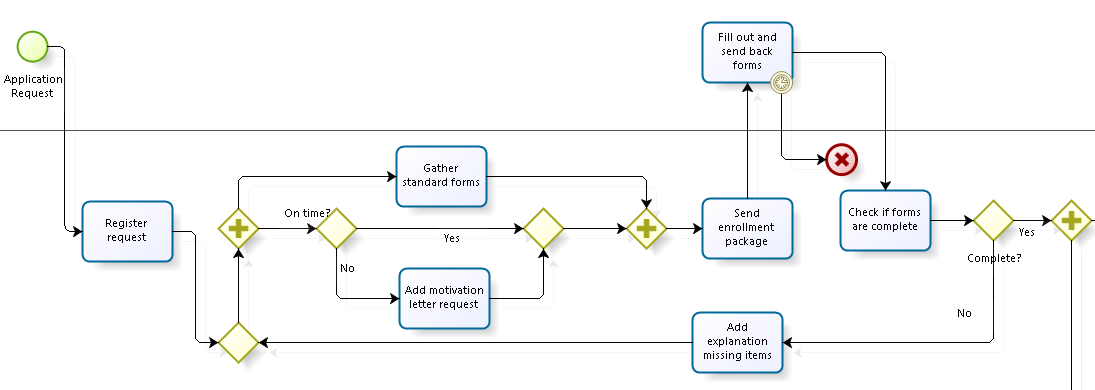
\includegraphics[scale=0.5]{model1-part1}
	\caption{The first part of the model in Bizagi}
	\label{fig:model1-part1}
\end{figure}

If the forms were all complete the process continues and up to three tasks are done simultaneously (depending if a motivation letter was required).
The first task is \emph{Check prerequisites}, in this task a administrative employee checks if all the general prerequisites are met.
If so, the process continues but has to wait until all three tasks are finished.
If the prerequisites are not met the next task in the process is \emph{Notify student}.
In this task a mail department employee notifies the student that his request has failed because some of the prerequisites are not met.
After this the process has terminated.

The second simultaneous task is \emph{Check financial prerequisites}.
In this task a financial department employee checks these prerequisites.
If these are not met, the same process flow as with the normal prerequisites is followed and the process terminates.
If met, the process has to wait for the (potential) last task.

The last task is optional. This task is \emph{Check motivation letter}.
This task needs only to be done if a motivation letter was required, so before a departmental executive board employee checks the motivation letter,
an automatic check is done to see if this task needs to be executed.
If not the process skips this task and the process can continue if the first two prerequisites checks are completed.
If the motivation letter was not good enough the process terminates again via the above mentioned way.
If the letter was good the process can continue if all three tasks are completed.

Though in the process description in \autoref{app:appendix_exercise} it is mentioned that these tasks take place after each other,
we choose to do them simultaneously because they need different resources and do not depend on each other.
This choice leads to a shorter process flow time, but a higher percentage of inefficient work.
This is because one of the checks might result in a failure.
In that case both the other checks should not have been done, but we value the flow time more than the efficiency.

\begin{figure}[H]
	\centering
	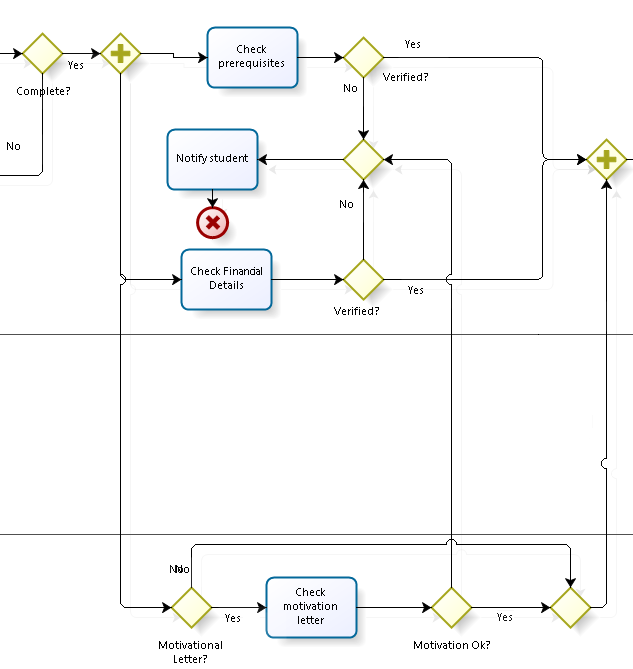
\includegraphics[scale=0.5]{model1-part2}
	\caption{The second part of the model in Bizagi}
	\label{fig:model1-part2}
\end{figure}

Once all the prerequisites are checked, the registration of the student cannot fail anymore.
At this point the process splits into two flows.
The first flow is the final part of the registration of a student and the second flow is the order and payment of the laptop.
We have explicitly chosen that a laptop is not ordered earlier than this, because otherwise it would be possible to order a laptop for a student and the registration of that student fails.
This would cause that the NSC could order too much laptops which would be expensive.

We shall describe the registration part first.
After the prerequisites check the process moves on to \emph{Register student}.
In this task the administrative employee registers the student at the university.
After that the departmental administrative employee registers the student in the study program of the department corresponding to the chosen study program.
This is all done in task \emph{Register student at Department}.
At last the student is notified by a mail department employee that the registration is complete via the task \emph{Notify Successful Registration}.
Important to note is that once this task is completed it is not possible anymore to pay for the laptop via a bank.
When this part of the process is completed, the process has to wait for the other part to finish before the process can terminate.

Now we handle the second part.
After the prerequisites were approved the process also continues to one of the tasks \emph{Order separate notebook} or \emph{Add notebook to Bulk order}.
Which one of the tasks will be executed depends on whether the registration was on time or not.
If it was on time than the task \emph{Add notebook to Bulk order} is executed and otherwise \emph{Order separate notebook} will be done.
Both these tasks are done by an employee of the Notebook Service Center, further on mentioned to as NSC employee.

Now the process continues to the task \emph{Notebook arrives}.
This is the task where a NSC employee receives the notebook(s).
When this task is finished, there are now three possible scenario's.
In the first scenario the student wants to pay via a bank and the registration is not yet completed.
In this case the process will continue to the task \emph{Payment via bank Student}.
In the second scenario the student wants to pay via a bank, but the registration is already completed.
In this case the process continues to the task \emph{Pay Laptop in Cash}, since it is not possible anymore to pay via bank.
In the third and last scenario the student wants to pay in cash and the process continues to \emph{Pay Laptop in Cash}.
The payment via the bank will be done automatically, but for the payment in cash we also need a NSC employee to receive the money.

After one of these two tasks are completed the process moves on to \emph{Pick up Laptop}.
In this task the NSC employee gives the laptop to the new student.
After this task, this part of the process is finished and if the registration is also finished the process can terminate, otherwise the process has to wait until the registration is complete.

\begin{figure}[H]
	\centering
	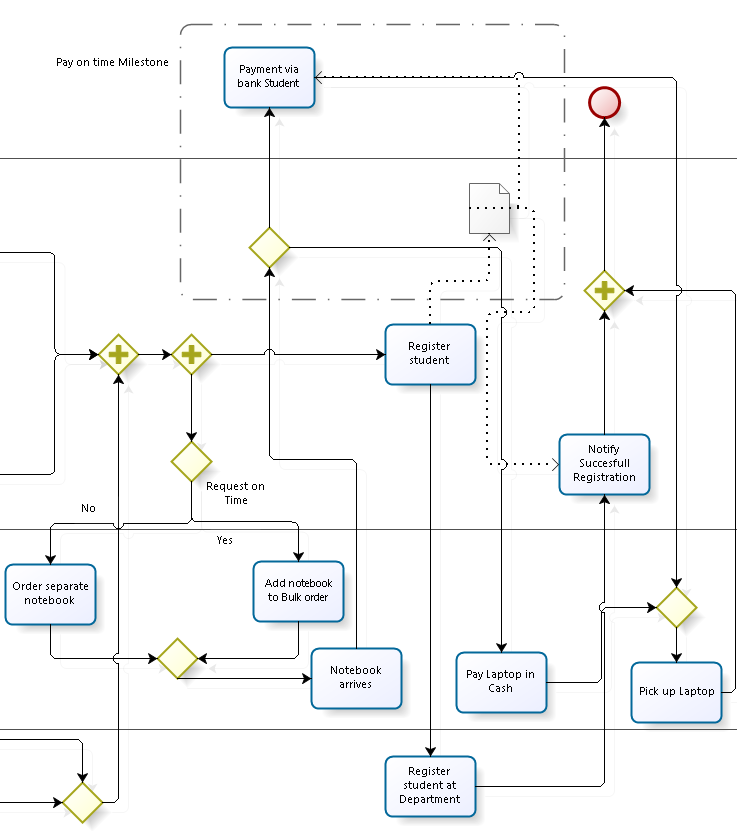
\includegraphics[scale=0.4]{model1-part3}
	\caption{The last part of the model in Bizagi}
	\label{fig:model1-part3}
\end{figure}

\subsection{Workflow patterns}

\subsubsection{Parallelism}

	Figure~\ref{fig:patterns:parallelism} shows the parallelism pattern used in our model.

	\begin{figure}[H]
		\centering
		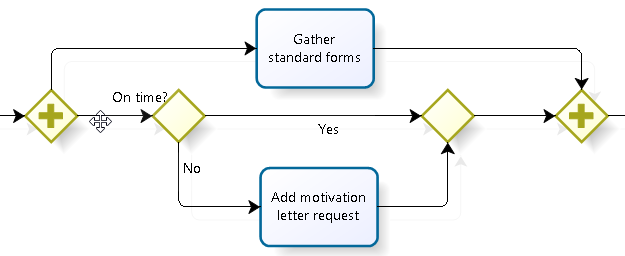
\includegraphics[width=0.8\textwidth]{pattern-parallel}
		\caption{Parallelism workflow pattern}
		\label{fig:patterns:parallelism}
	\end{figure}

	We use parallelism here to decrease the flow time and increase resource utilisation.
	Since gathering standard forms and adding a letter to the mail package can be done at the same time, the total time required to finish this part of the flow can be lower.

\subsubsection{Implicit XOR-split}

	Figure~\ref{fig:patterns:implxor} shows the implicit XOR-split pattern used in our model.

	\begin{figure}[H]
		\centering
		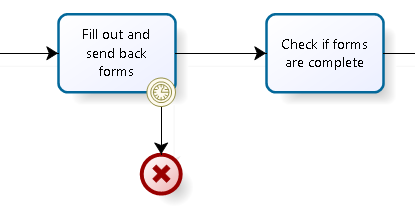
\includegraphics[width=0.7\textwidth]{pattern-implxor}
		\caption{Implicit XOR-split workflow pattern}
		\label{fig:patterns:implxor}
	\end{figure}

	We use the deferred timer choice to end the model when the applicant does not reply on time.

\subsubsection{Explicit XOR-split}

	Figure~\ref{fig:patterns:explxor} shows the explicit XOR-split pattern used in our model.

	\begin{figure}[H]
		\centering
		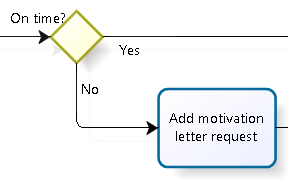
\includegraphics[width=0.5\textwidth]{pattern-explxor}
		\caption{Explicit XOR-split workflow pattern}
		\label{fig:patterns:explxor}
	\end{figure}

	The explicit XOR-split is used a number of times throughout the model to make direct choices based on user input or state.
	In this case, we use it do decide whether or not it's necessary to add a request for a motivation letter.

\subsubsection{OR-join}

	Figure~\ref{fig:patterns:orjoin} shows the OR-join pattern used in our model.

	\begin{figure}[H]
		\centering
		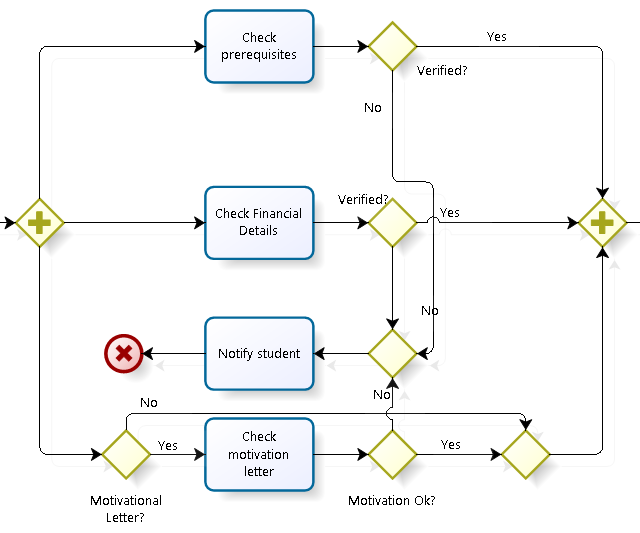
\includegraphics[width=0.9\textwidth]{pattern-orjoin}
		\caption{OR-join workflow pattern}
		\label{fig:patterns:orjoin}
	\end{figure}

	We model the OR-join pattern as a parallel split with choices.
	In Figure~\ref{fig:patterns:orjoin}, we make use of this pattern for the different types of checks on the applicant.

\subsubsection{Iteration}

	Figure~\ref{fig:patterns:iteration} shows the iteration pattern used in our model.

	\begin{figure}[H]
		\centering
		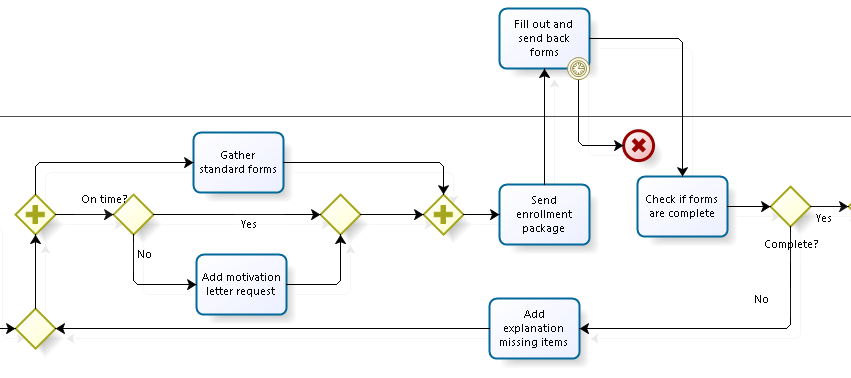
\includegraphics[width=\textwidth]{pattern-iteration}
		\caption{Iteration workflow pattern}
		\label{fig:patterns:iteration}
	\end{figure}

	Our implementation of the iteration pattern is a simple loop that will repeat the information gathering part of the model.
	If an applicant does not fill out the forms completely, we step back to sending the enrollment package.

\subsubsection{Milestone}

	Figure~\ref{fig:patterns:milestone} shows the milestone pattern used in our model.

	\begin{figure}[H]
		\centering
		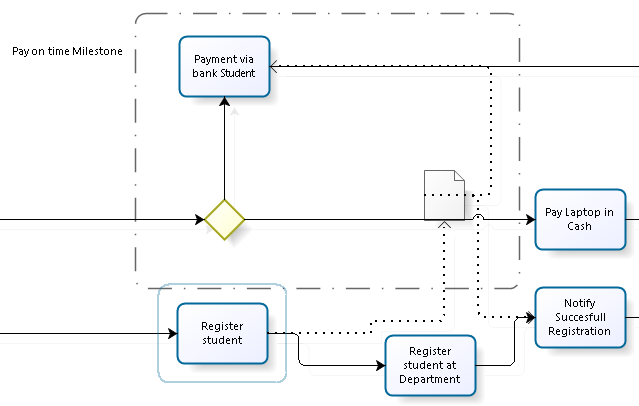
\includegraphics[width=\textwidth]{pattern-milestone}
		\caption{Milestone workflow pattern}
		\label{fig:patterns:milestone}
	\end{figure}

	We use the milestone pattern to make sure that applicants can only pay via bank transfer while the registration is still running.
	After the registration is complete, applicants can only pay in cash.
